\documentclass[12pt,letterpaper]{article}
\usepackage{amsmath}
\usepackage{gensymb}
\usepackage{enumitem}
\usepackage{graphicx}
\usepackage[margin=1in]{geometry}
\setlength{\parindent}{0pt}
\title{Physics Club Practice Test 2}
\usepackage[export]{adjustbox}
\usepackage[none]{hyphenat}
\usepackage{titlesec}
\titlespacing{\section}{0pt}{4.0ex plus .2ex}{-3.3ex}
\titlespacing{\paragraph}{0pt}{0pt}{1em}
% \setenumerate[2]{label={\alph*.}}
\usepackage{fancyhdr}
\fancypagestyle{firstpage}
{
	\renewcommand{\headrulewidth}{0pt}
	\renewcommand{\footrulewidth}{0.4pt}
	\lfoot{Physics Club}
	\cfoot{$F=ma$ Practice Test 2}
	\rfoot{\thepage}
}
\thispagestyle{firstpage}
\pagestyle{fancy}
\fancyhf{}
\renewcommand{\headrulewidth}{0pt}
\renewcommand{\footrulewidth}{0.4pt}
\lfoot{Physics Club}
\cfoot{$F=ma$ Practice Test 2}
\rfoot{\thepage}
\begin{document}
\section*{Physics Club: $F=ma$ Practice Test 2}\hfill Version 1.0
\vspace{-2.5pt}
\begin{center}
\textsc{25 Questions -- 75 Minutes}
\end{center}
\vspace{-5pt}
Assume the acceleration due to gravity near the surface of the Earth $g = 10$ m/s$^2$.
\smallskip

Correct answers will be awarded one point; incorrect answers will result in a deduction of 1/4 point. There is no penalty for leaving an answer blank.
\smallskip

You may use a scientific calculator. Its memory must be cleared of data and programs.

\vspace{-5pt}
\hrulefill
\vspace{-10pt}

\begin{enumerate}

\item
A cannon simultaneously fires two identical cannonballs at targets 1 and 2 as shown below. If the cannonballs have identical initial speeds, which one of the following statements is true? Neglect air resistance.

\begin{tabular}{l r}

\begin{minipage}{0.5\textwidth}
\begin{enumerate}
\item Target 1 is hit before target 2.
\item Target 2 is hit before target 1.
\item Both are hit at the same time.
\item Which target gets hit first cannot be determined exactly.
\item The kinetic energy of the cannonball that strikes target 1 must be greater than the kinetic energy of the ball that strikes target 2.
\end{enumerate}
\end{minipage} &
\begin{minipage}{0.4\textwidth}
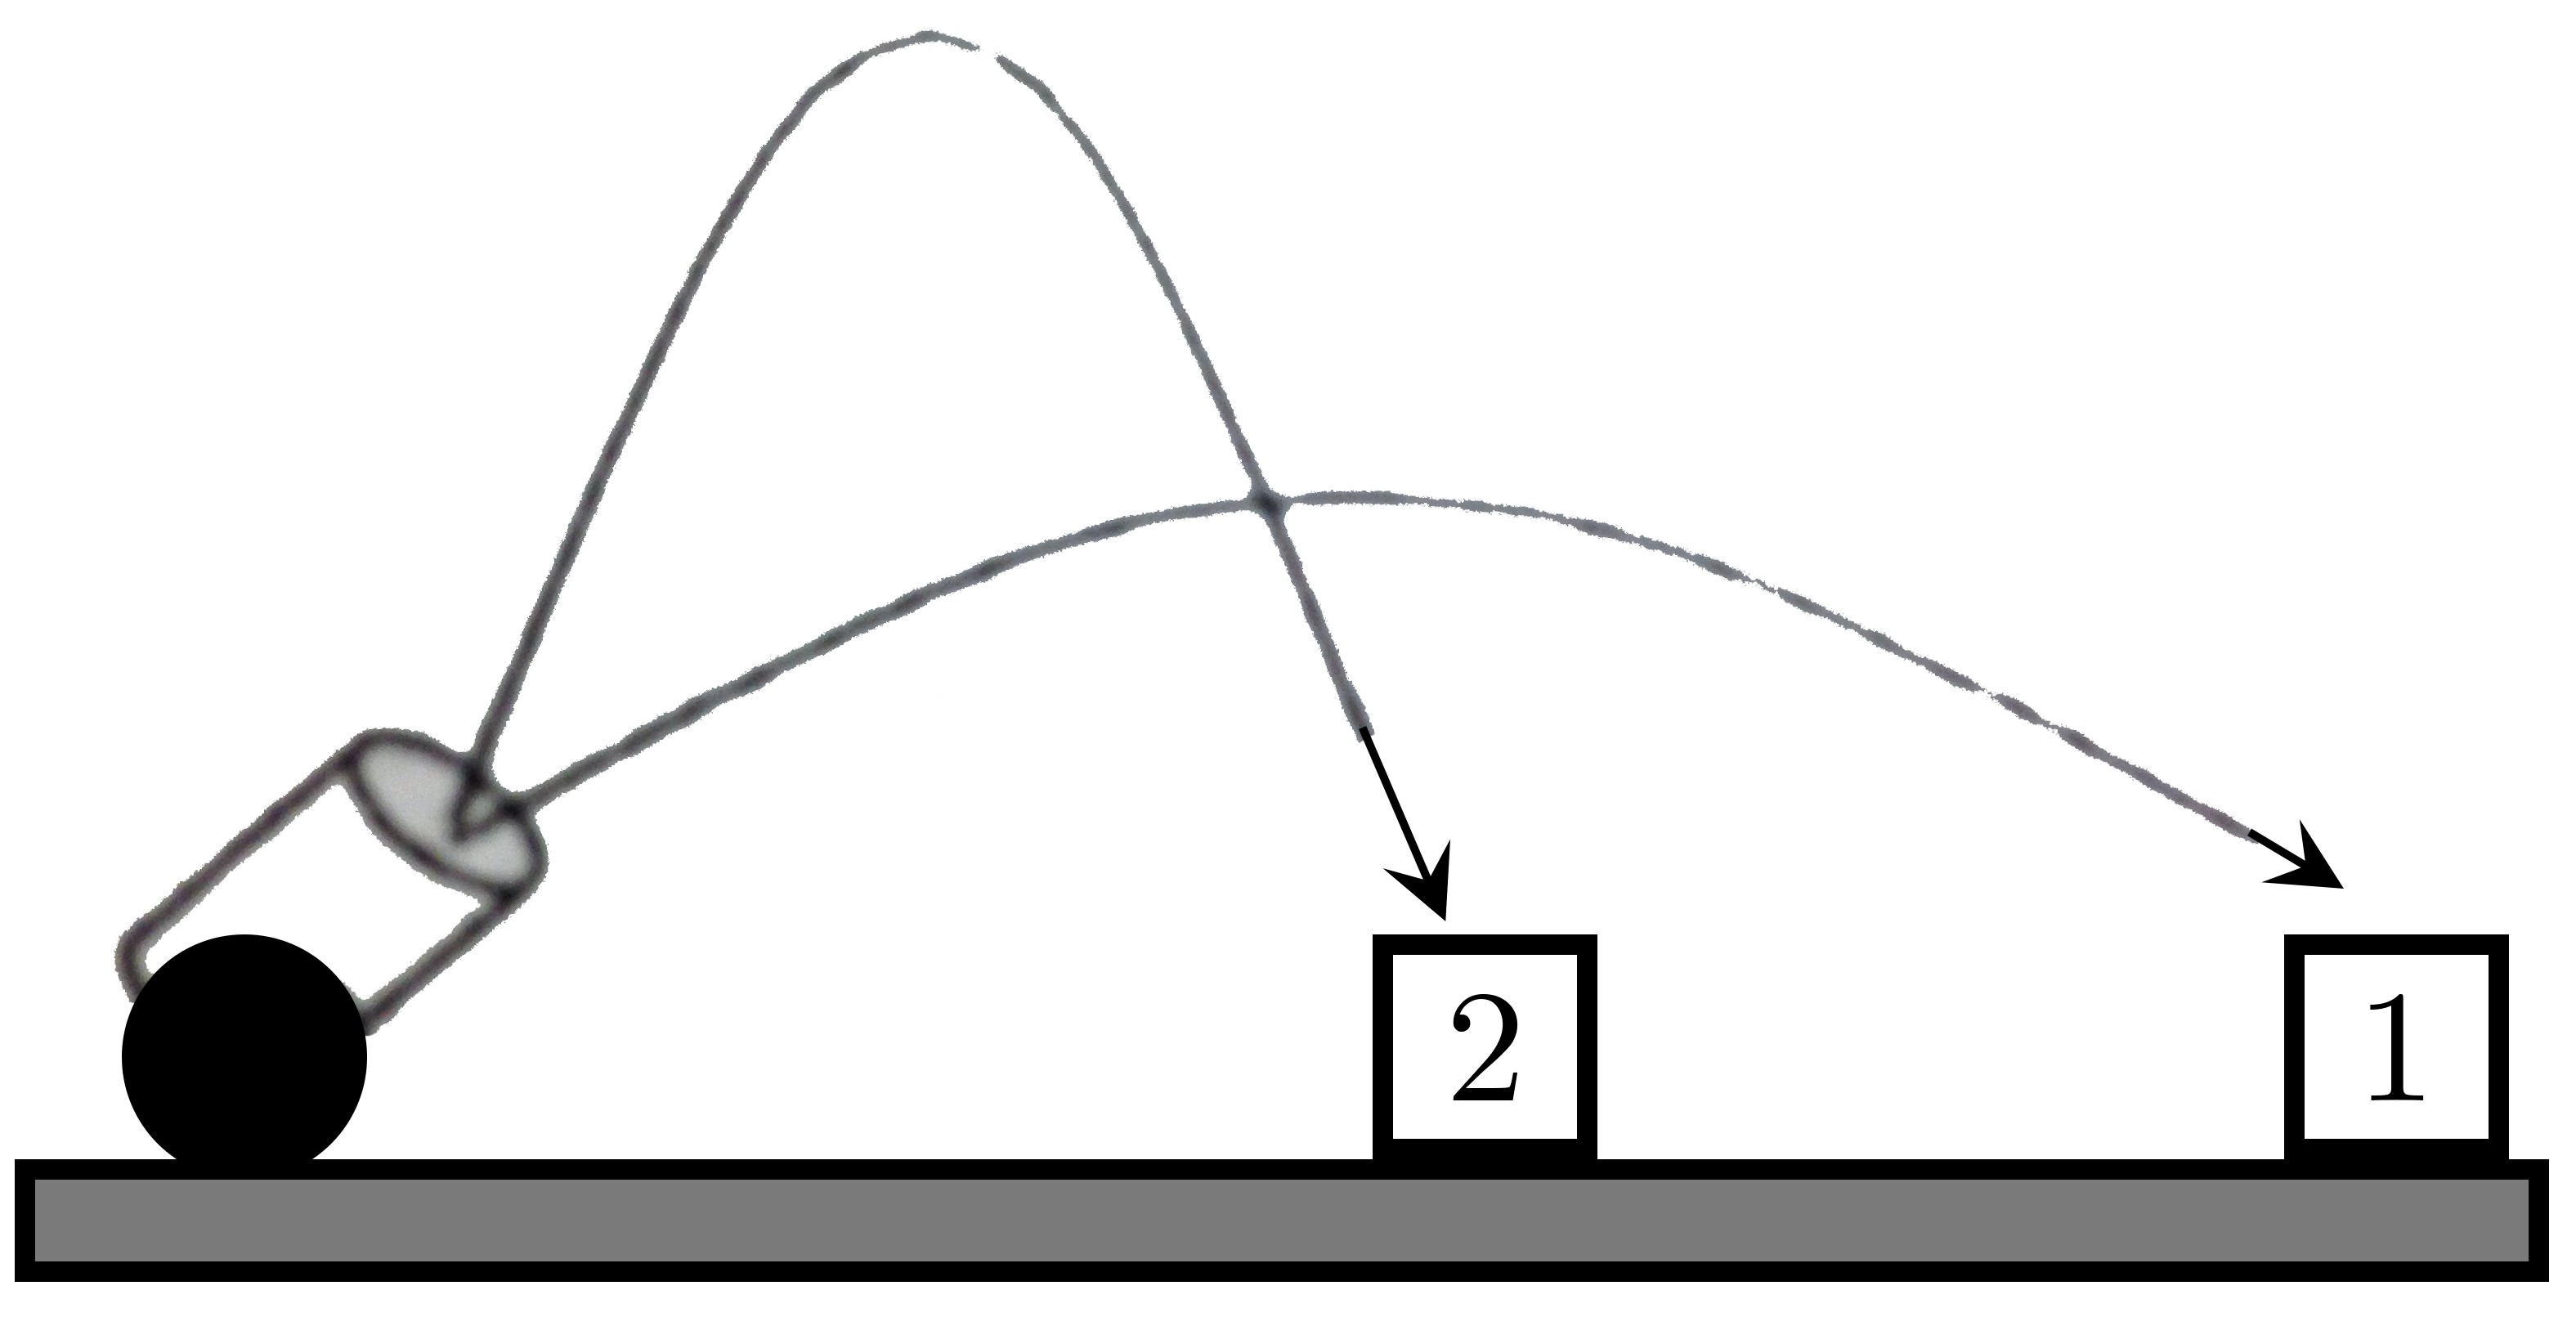
\includegraphics[width=\textwidth]{cannon.png}
\end{minipage}
\end{tabular}

\item
A large truck and a small car collide and stick together. The change in momentum of which one is larger in magnitude?
\begin{enumerate}
\item The car
\item The truck
\item The momentum change is the same for both vehicles
\item Cannot tell without knowing the final velocity of the combined mass
\item Cannot tell without knowing the masses of the truck and the car
\end{enumerate}

\item
A glass bottle falls off a table onto the floor and breaks into pieces. Which of the following statements regarding the process is \emph{incorrect}?
\begin{enumerate}
\item The potential energy of the bottle has changed.
\item Some of the potential energy of the bottle has eventually been converted into the energy to break the bottle.
\item Some of the kinetic energy of the bottle has eventually been converted into the energy to break the bottle.
\item The impulse from the floor to the bottle is larger in magnitude than the impulse from the bottle to the floor.
\item The impact from the floor to the bottle breaks the bottle.
\end{enumerate}

\item
The kinetic energy of a particle in a simple harmonic motion is $\frac{1}{2}av^2$, its potential energy is $\frac{1}{2}bx^2$, where $x$ is the coordinate for the position of the particle and $v$ is its seed. Find the frequency of the motion.
\begin{enumerate}
\item $\displaystyle \frac{1}{2\pi}\sqrt\frac{a}{b}$
\item $\displaystyle \frac{1}{2\pi}\sqrt\frac{b}{a}$
\item $\displaystyle \frac{1}{2\pi}\sqrt{\frac{a}{b}+\frac{b}{a}}$
\item $\displaystyle \frac{1}{2\pi}\sqrt{ab}$
\item $\displaystyle \frac{1}{2\pi}\sqrt\frac{1}{ab}$
\end{enumerate}

\item
Two teams of movers are lowering a piano from the window of a 20 floor apartment building. The rope breaks when the piano is 50 meters above the ground. The movers on the ground, alerted by the shouts of the movers above, first notice the piano when it is 30 meters above the ground. How long do they have to get out of the way before the piano hits the ground?
\begin{enumerate}
\item 0.66 s
\item 0.78 s
\item 1.2 s
\item 1.8 s
\item 2.5 s
\end{enumerate}

% --- F=ma Question ---
% \item
% A ball with mass $m$ is projected horizontally off the end of a table with an initial kinetic energy $K$. At a time $t$ after it leaves the end of the table, it has kinetic energy $4K$. What is $t$? Neglect air resistance.
% \begin{enumerate}
% \item $\displaystyle \frac{3}{g}\sqrt\frac{K}{m}$
% \item $\displaystyle \frac{2}{g}\sqrt\frac{K}{m}$
% \item $\displaystyle \frac{1}{g}\sqrt\frac{6K}{m}$
% \item $\displaystyle \frac{K}{g}\sqrt\frac{6}{m}$
% \item $\displaystyle \frac{2K}{g}\sqrt\frac{1}{m}$
% \end{enumerate}

\item
The diagram shows an oscillating trolley. The frequency of the oscillations can be substantially increased by

\begin{tabular}{l r}

\begin{minipage}{0.4\textwidth}
\begin{enumerate}
\item increasing the amplitude of the oscillations.
\item fixing an extra mass to the trolley.
\item reducing the effect of friction on the trolley.
\item linking the trolley to the supports with a stronger pair of springs.
\item none of the above.
\end{enumerate}
\end{minipage} &
\begin{minipage}{0.5\textwidth}
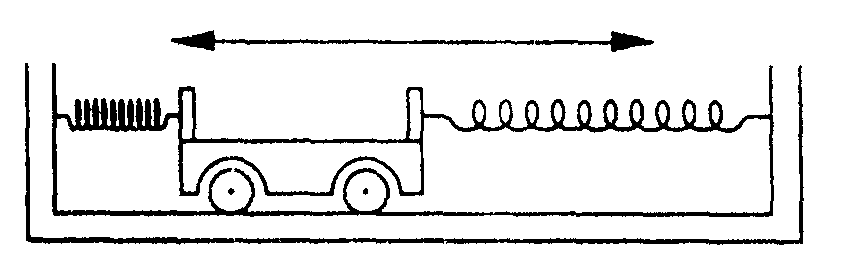
\includegraphics[width=\textwidth]{trolley.png}
\end{minipage}
\end{tabular}

\vfill
\newpage

\item
A block moves toward the right with a uniform deceleration along a rough horizontal surface as shown in the diagram below.

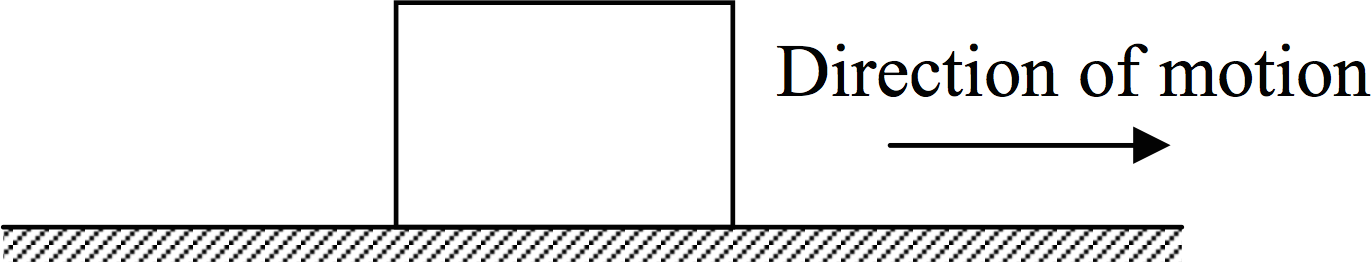
\includegraphics[width=0.5\textwidth,center]{block-q-lg.png}
Neglecting air resistance, which one of the following diagrams correctly shows the lines of application of all the forces acting on the block? (The dot represents the block's center of mass.)

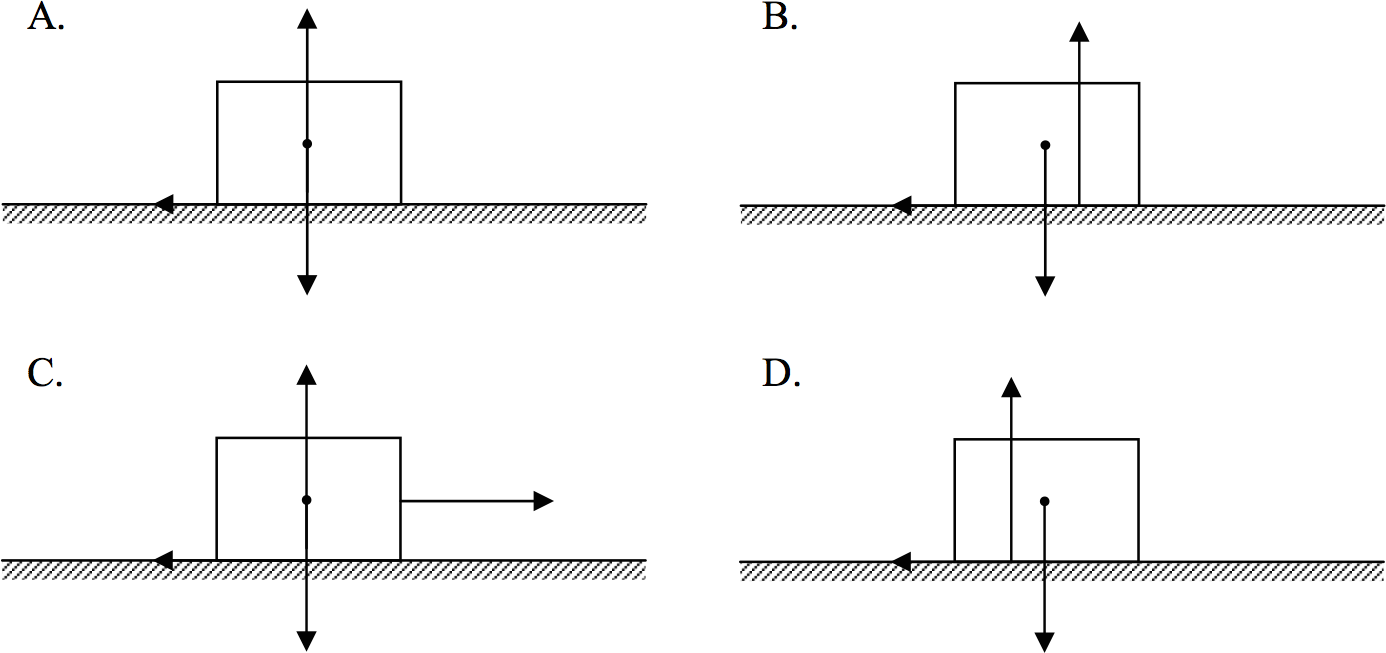
\includegraphics[width=0.9\textwidth,center]{block-ans.png}
\begin{enumerate}
\setcounter{enumii}{4}
\item Either (c) or (d) can be correct
\end{enumerate}

\item
Two skaters on a frictionless icy surface push apart from one another. The first skater has a mass $M$ which is greater than the mass $m$ of the second skater. After some time the two skaters are at a distance $d$ apart. How far has the lighter skater moved from her original position?
\begin{enumerate}[itemsep=10pt]
\item $\displaystyle \frac{M}{m}d$
\item $\displaystyle \frac{m}{M}d$
\item $d$
\item $\displaystyle \frac{m}{M+m}d$
\item $\displaystyle \frac{M}{M+m}d$
\end{enumerate}

\vfill
\newpage

\item
An opened parachute of mass 1.0 kg is coming straight down from the sky. Attached to the parachute is the upper end of a light spring scale, while a block of mass 10 kg is attached to the lower end of the scale. The scale reading is 80 N. The air resistance at the moment is approximately
\begin{enumerate}
\item 55 N.
\item 66 N.
\item 77 N.
\item 88 N.
\item 99 N.
\end{enumerate}

\item
As shown in the figure, a hemispherical bowl is placed horizontally on a table. Point O is the center of the hemisphere. The edge and the surface of the bowl are smooth. A particle of mass $m_1$ is placed in a bowl and is tied to a string with negligible mass. The other end of the string is tied to another particle of mass $m_2$ hanging outside the bowl. When the system is in equilibrium, the line joining the particle $m_1$ and point O makes an angle $\alpha = 60\degree$ with the horizontal. Find the ratio $m_1/m_2$.

\begin{tabular}{l r}

\begin{minipage}{0.6\textwidth}
\begin{enumerate}
\item 0.71
\item 0.87
\item 1.15
\item 1.41
\item 1.73
\end{enumerate}
\end{minipage} &
\begin{minipage}{0.3\textwidth}
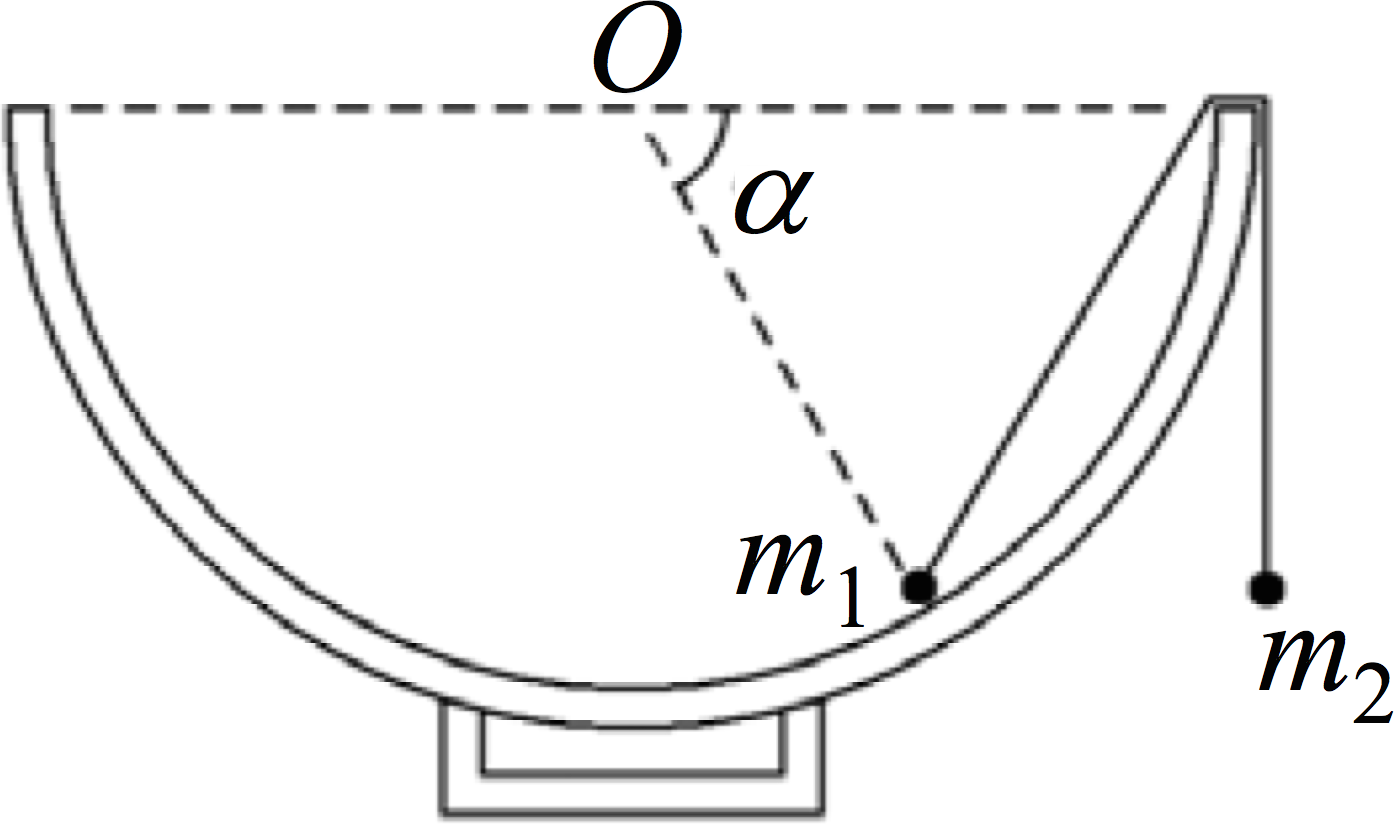
\includegraphics[width=\textwidth]{bowl.png}
\end{minipage}
\end{tabular}

\item
As shown, one end of a light thread is fixed on the ceiling and the other end tied to a small sphere. The angle between the thread and the vertical direction is $\beta$. When $\beta = \alpha$ and $\alpha$ is a small angle, the sphere is in simple harmonic motion like a pendulum with period $T$. When $\beta = \alpha_1$ or $\alpha_2$ ($\alpha < \alpha_1 < \alpha_2$), the sphere is in a uniform circular motion in a horizontal plane with period $T_1$ or $T_2$, respectively. Then the correct relation is

\begin{tabular}{l r}

\begin{minipage}{0.7\textwidth}
\begin{enumerate}
\item $T < T_1 < T_2$.
\item $T = T_1 = T_2$.
\item $T > T_1 > T_2$.
\item $T_1 < T < T_2$.
\item $T_1 > T > T_2$.
\end{enumerate}
\end{minipage} &
\begin{minipage}{0.2\textwidth}
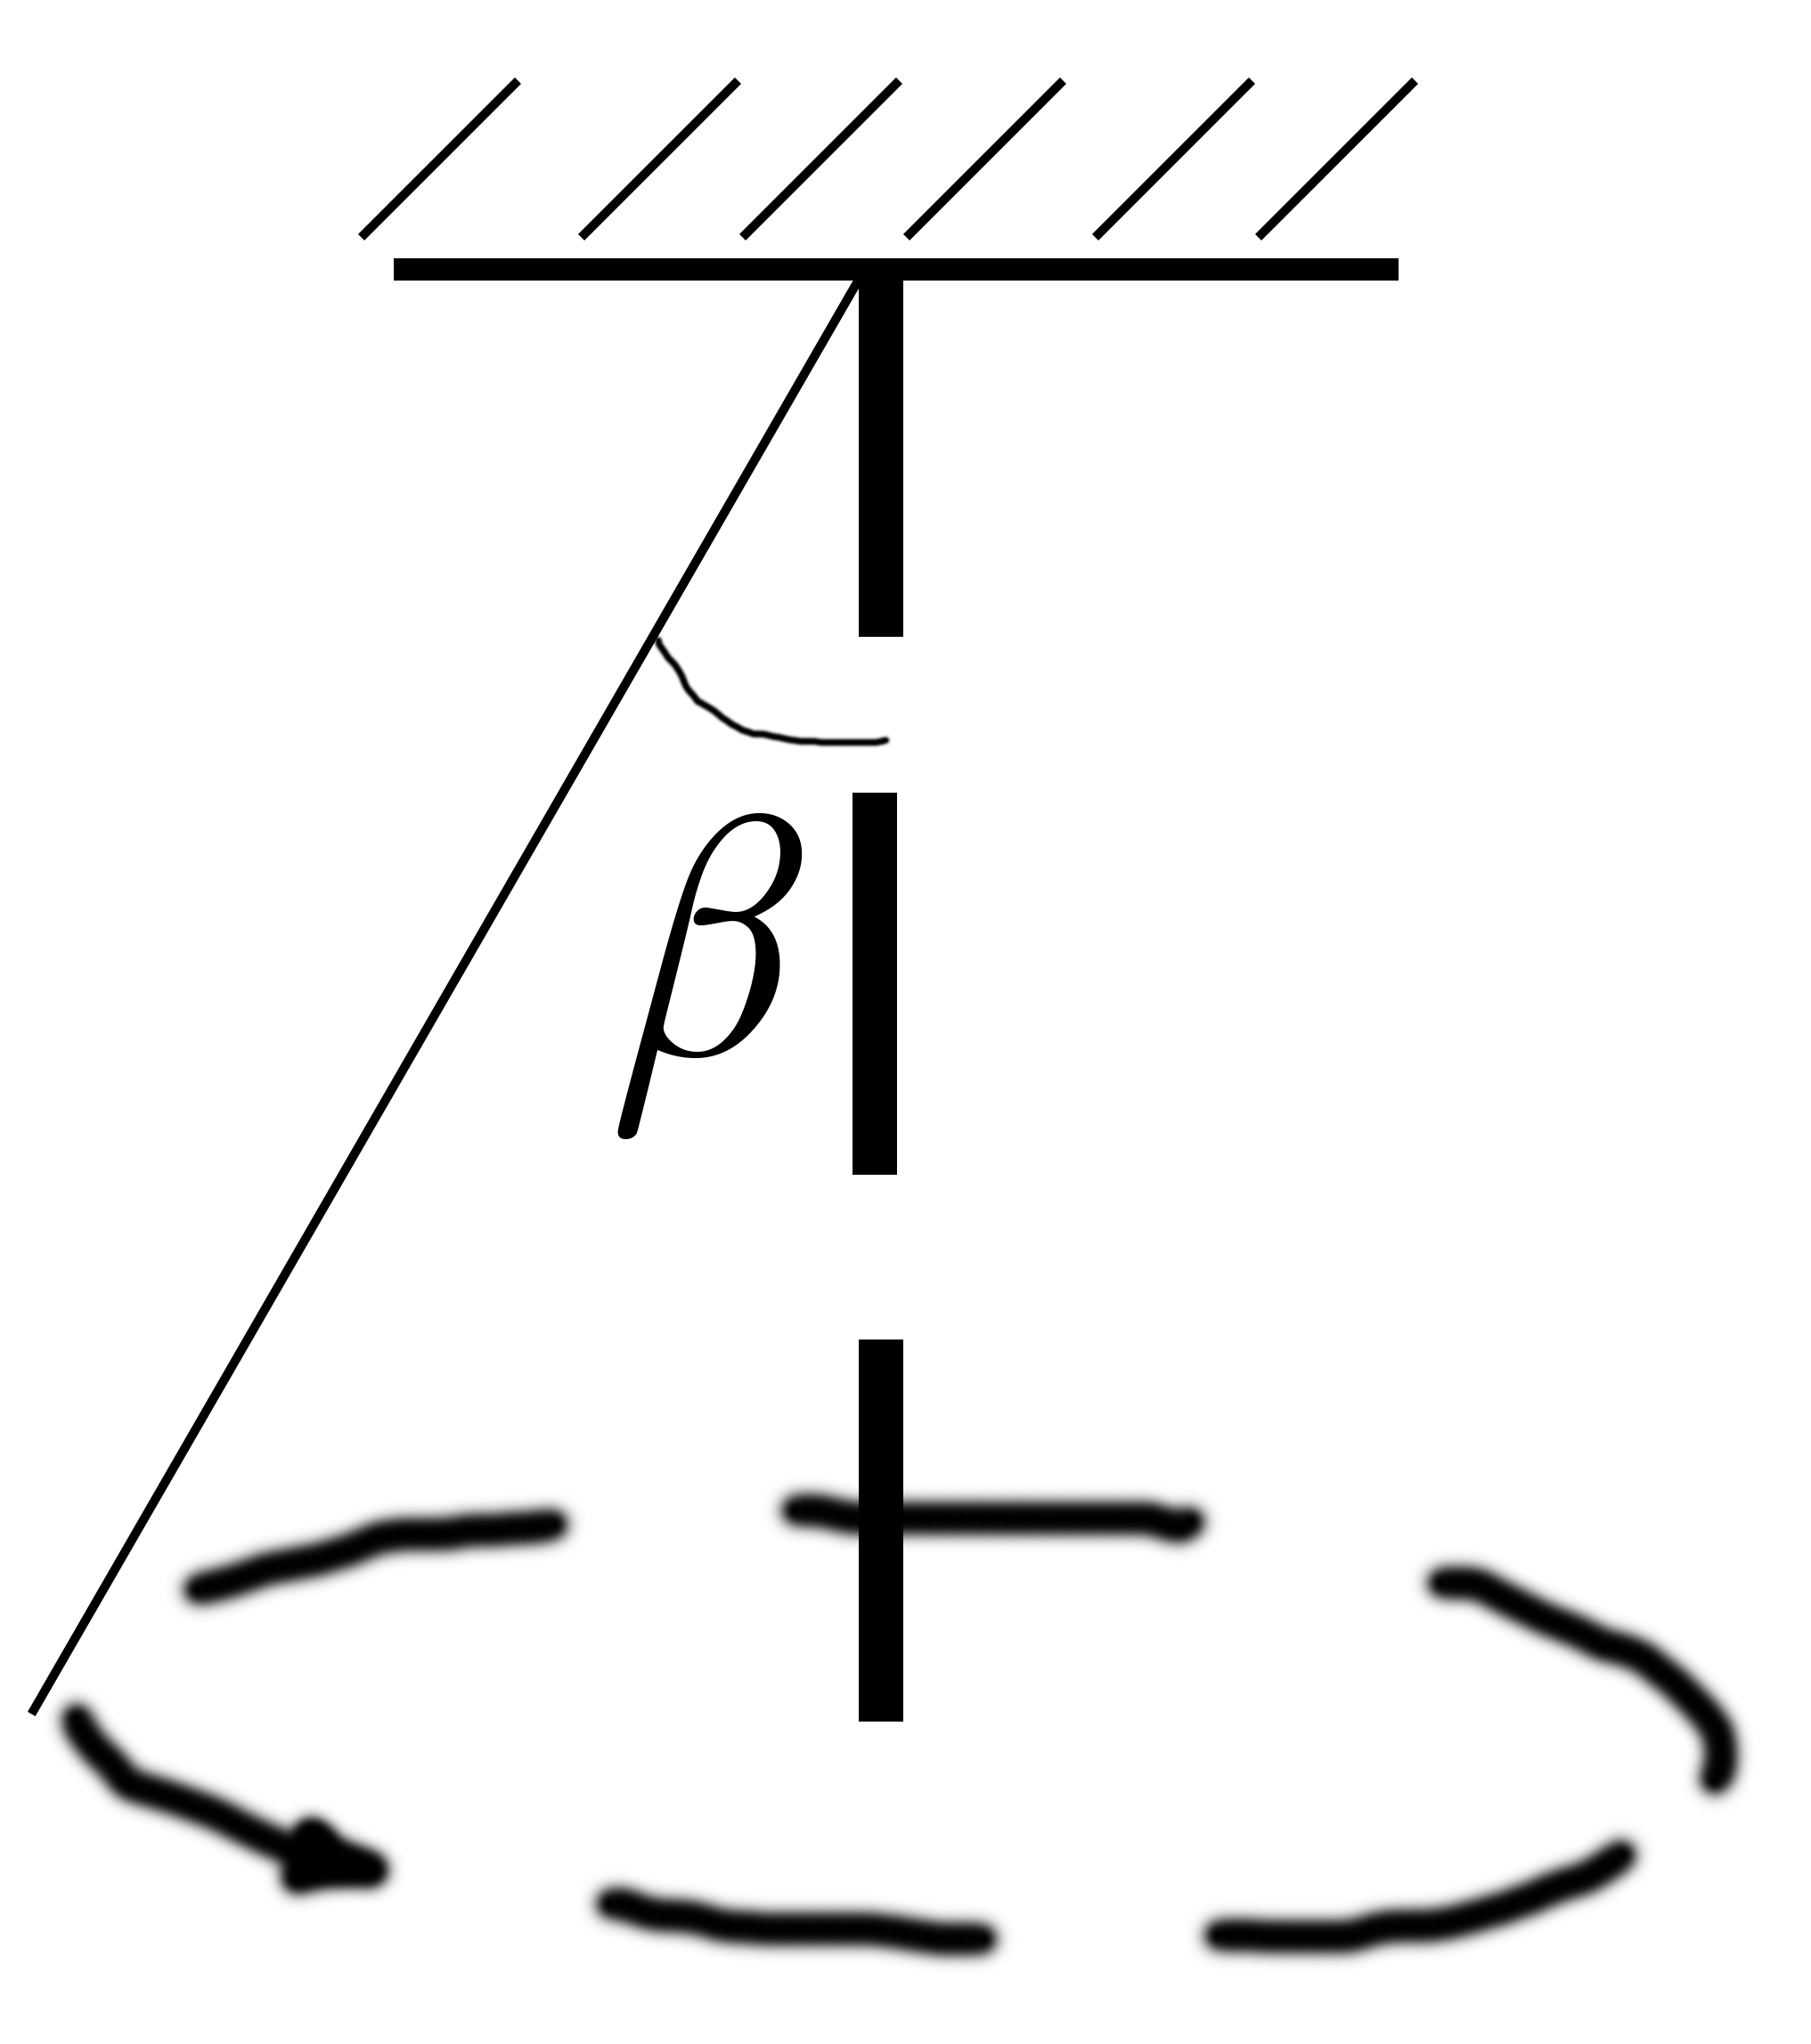
\includegraphics[width=\textwidth]{pendulum.png}
\end{minipage}
\end{tabular}

\vfill
\newpage

\item
A small wooden sphere of density 0.8 g/cm$^3$ is attached to the end of a string of length 4.0 m in water. The other end of the string is attached to the bottom, forming a reverse pendulum. Ignore water friction. Find the period of the pendulum.
\begin{enumerate}
\item 4 s
\item 2 s
\item 5 s
\item 1 s
\item 8 s
\end{enumerate}

\item
A stream of water of density $\rho$, cross-sectional area $A$, and speed $v$ strikes a wall at a height $h$ from the ground. The wall is perpendicular to the direction of the stream, as shown in the figure below. The water then flows sideways across the wall. The force exerted by the stream on the wall is

\begin{tabular}{l r}

\begin{minipage}{0.7\textwidth}
\begin{enumerate}
\item $2\rho v^2A$.
\item $\rho v^2A$.
\item $\rho ghA$.
\item $\displaystyle \frac{v^2A}{\rho}$.
\item $\displaystyle \frac{v^2A}{2\rho}$.
\end{enumerate}
\end{minipage} &
\begin{minipage}{0.2\textwidth}
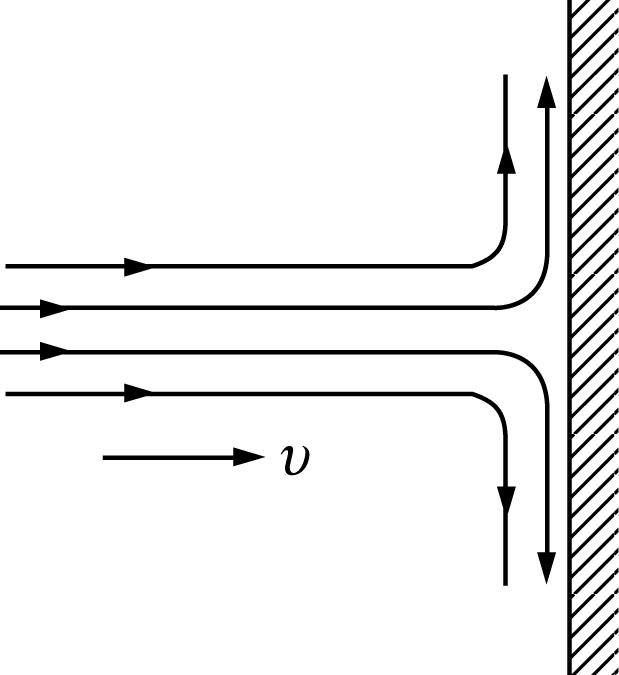
\includegraphics[width=\textwidth]{stream.png}
\end{minipage}
\end{tabular}

\item
A block of mass $M_1$ is hung by a light spring of force constant $k$ to the top bar of a reverse U-frame of mass $M_2$ on the floor. The block is pooled down from its equilibrium position by a distance $x$ and then released. Find the minimum value of $x$ such that the reverse U-frame will leave the floor momentarily.

\begin{tabular}{l r}

\begin{minipage}{0.6\textwidth}
\begin{enumerate}
\item $\displaystyle \left(M_1 + M_2\right)\frac{g}{k}$
\item $\displaystyle \left(2M_1 + M_2\right)\frac{g}{k}$
\item $\displaystyle \left(M_1 + 2M_2\right)\frac{g}{k}$
\item $\displaystyle M_1\frac{g}{k}$
\item $\displaystyle M_2\frac{g}{k}$
\end{enumerate}
\end{minipage} &
\begin{minipage}{0.3\textwidth}
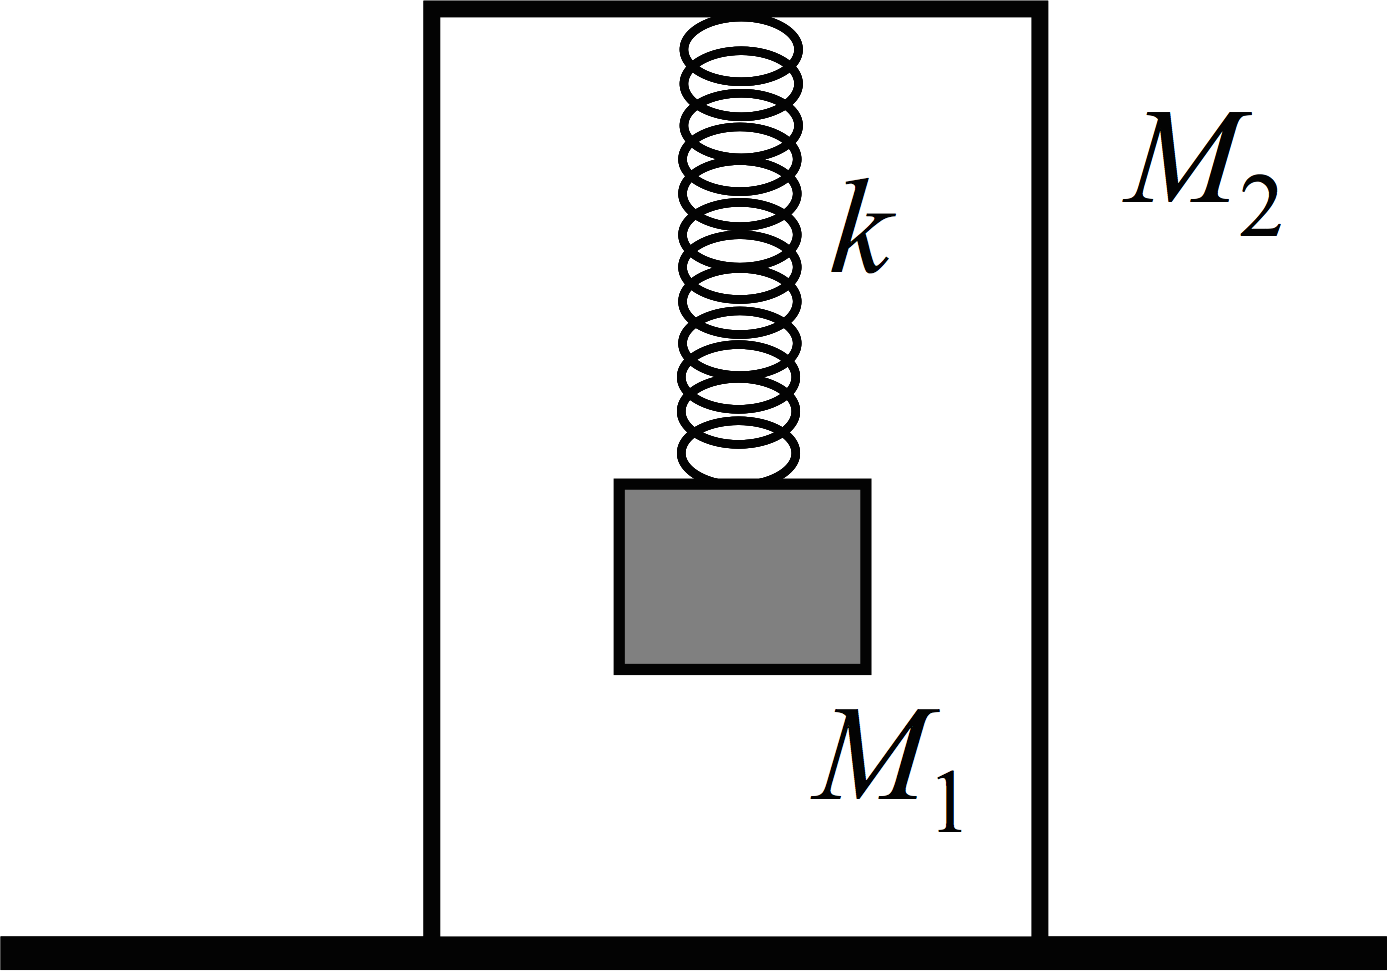
\includegraphics[width=\textwidth]{spring.png}
\end{minipage}
\end{tabular}

\vfill
\newpage

\item
As shown in the figure, two blocks of masses $m_1$ and $m_2$ are connected by a light string, and are placed on a horizontal smooth surface. Forces of magnitude $F_1$ and $F_2$ act on them respectively, causing them to move linearly. The force constant of the light string is $k$, and $F_1 > F_2$. What is the extension $x$ of the light string?

\begin{tabular}{l r}

\begin{minipage}{0.6\textwidth}
\begin{enumerate}
\item $\displaystyle \frac{F_1m_1+F_2m_2}{k(m_1+m_2)}$
\item $\displaystyle \frac{F_1m_2+F_2m_1}{k(m_1+m_2)}$
\item $\displaystyle \frac{|F_1m_2-F_2m_1|}{k(m_1+m_2)}$
\item $\displaystyle \frac{|F_1m_1-F_2m_2|}{k(m_1+m_2)}$
\item $\displaystyle \frac{F_1m_1+F_2m_2}{k|m_1-m_2|}$
\end{enumerate}
\end{minipage} &
\begin{minipage}{0.3\textwidth}
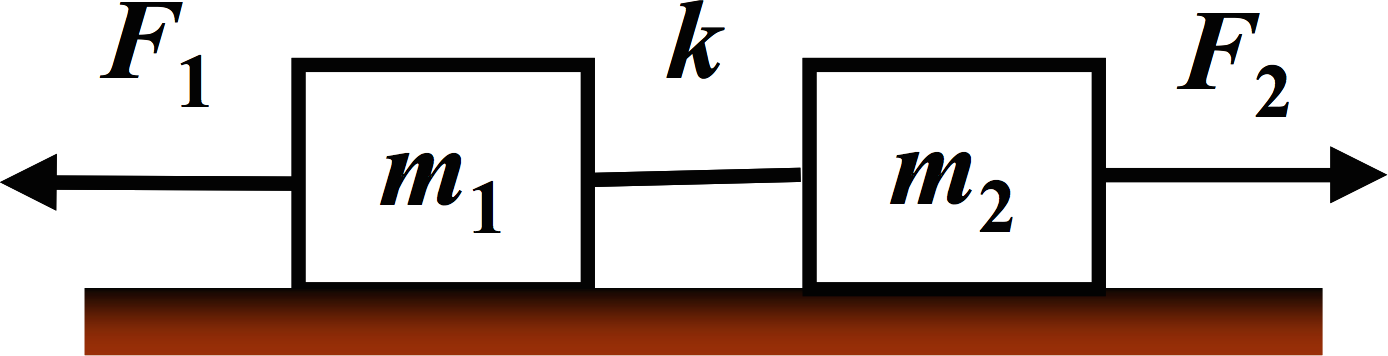
\includegraphics[width=\textwidth]{extension.png}
\end{minipage}
\end{tabular}

\item
A U-tube of small and uniform cross section contains water of total length $4H$. The height difference between the water columns on the left and on the right is $H$ when the valve K is closed. The valve is suddenly open, and water is flowing from left to right. Ignore friction. Find the speed of water when the heights of the left and the right water columns are the same.

\begin{tabular}{l r}

\begin{minipage}{0.5\textwidth}
\begin{enumerate}
\item $\displaystyle \frac{1}{4}\sqrt{gH}$
\item $\displaystyle \sqrt\frac{gH}{8}$
\item $\displaystyle \frac{1}{2}\sqrt{gH}$
\item $\displaystyle \sqrt\frac{gH}{2}$
\item $\sqrt{gH}$
\end{enumerate}
\end{minipage} &
\begin{minipage}{0.4\textwidth}
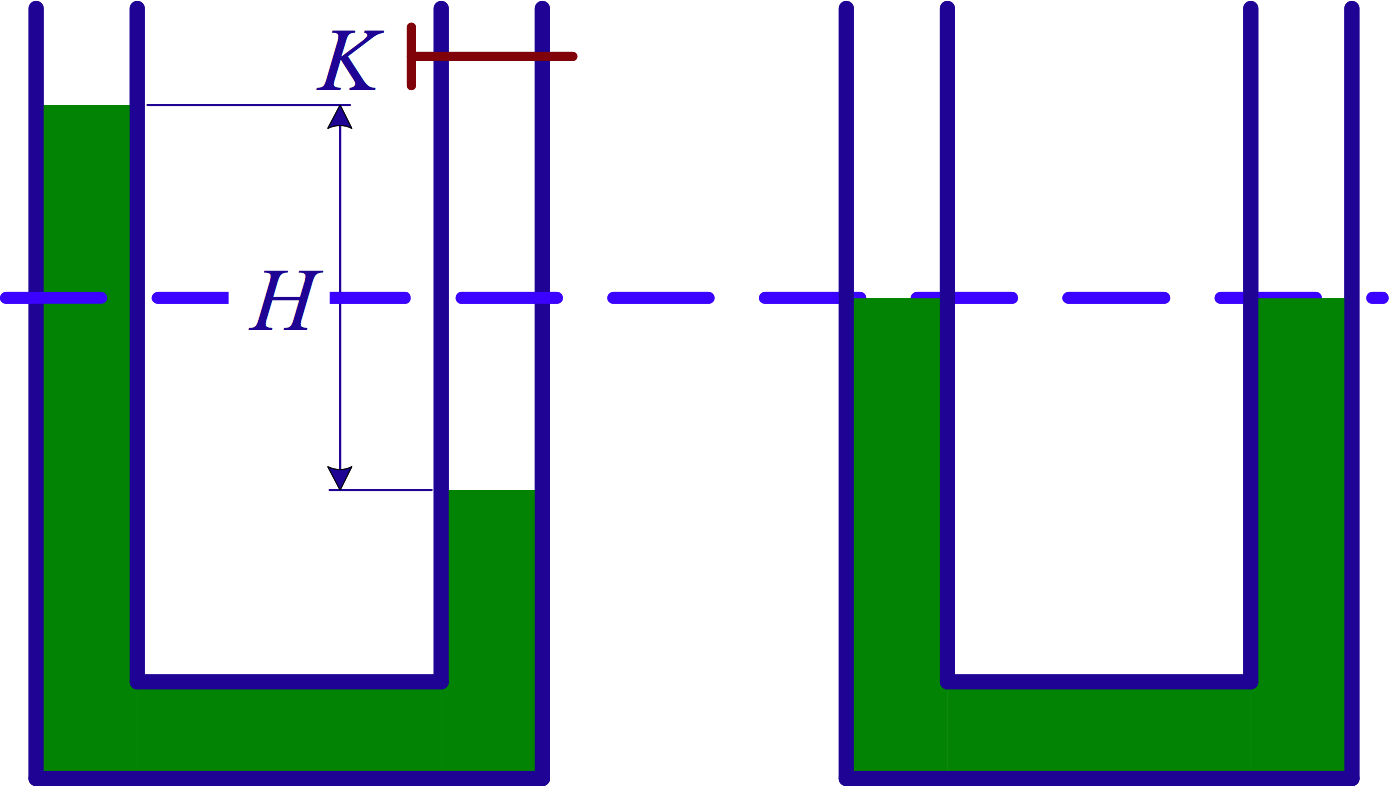
\includegraphics[width=\textwidth]{utube.png}
\end{minipage}
\end{tabular}

\vfill
\newpage

\item
Two blocks of mass $m_1 = 2$ kg and $m_2 = 4$ kg are suspended by two light strings to the ceiling as shown in the accompanying figure. If the upper string is suddenly broken, the accelerations of $m_1$ and $m_2$ at the moment when the upper string is broken are, respectively,

\begin{tabular}{l r}

\begin{minipage}{0.8\textwidth}
\begin{enumerate}
\item $a_1 = 10$ m/s$^2$ and $a_2 = 0$ m/s$^2$.
\item $a_1 = 10$ m/s$^2$ and $a_2 = 10$ m/s$^2$.
\item $a_1 = 20$ m/s$^2$ and $a_2 = 0$ m/s$^2$.
\item $a_1 = 20$ m/s$^2$ and $a_2 = 10$ m/s$^2$.
\item $a_1 = 30$ m/s$^2$ and $a_2 = 0$ m/s$^2$.
\end{enumerate}
\end{minipage} &
\begin{minipage}{0.1\textwidth}
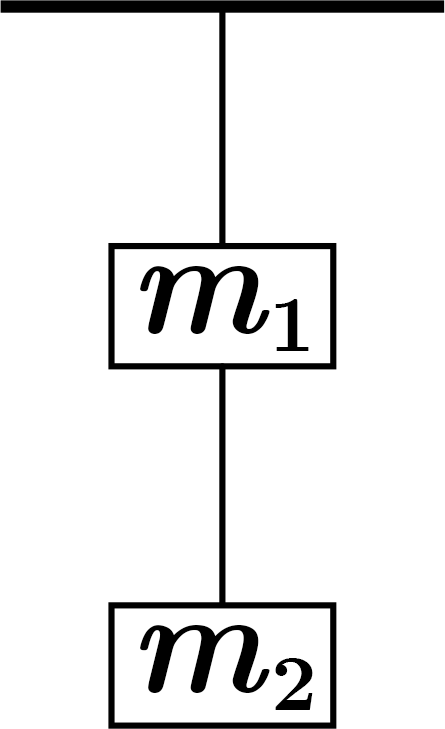
\includegraphics[width=\textwidth]{suspension.png}
\end{minipage}
\end{tabular}

\item
As shown in the figure, AB is a board of mass $M = 4$ kg and length $s = 2$ m, placed on a smooth horizontal surface. A bumper of negligible mass is fixed at end B. A peg of mass $m = 1$ kg is placed at end A. The coefficient of kinetic friction between the peg and the board is $\mu = 0.2$. With the board initially at rest, the peg is ejected with an initial velocity of $v_0 = 10$ m/s along the board surface. The peg is in contact with the board until it hits the bumper at end B. After the collision, the peg is just able to return to end A without falling off the board, Find the mechanical energy lost in the process.

\begin{tabular}{l r}

\begin{minipage}{0.4\textwidth}
\begin{enumerate}
\item 20 J
\item 24 J
\item 28 J
\item 32 J
\item 40 J
\end{enumerate}
\end{minipage} &
\begin{minipage}{0.5\textwidth}
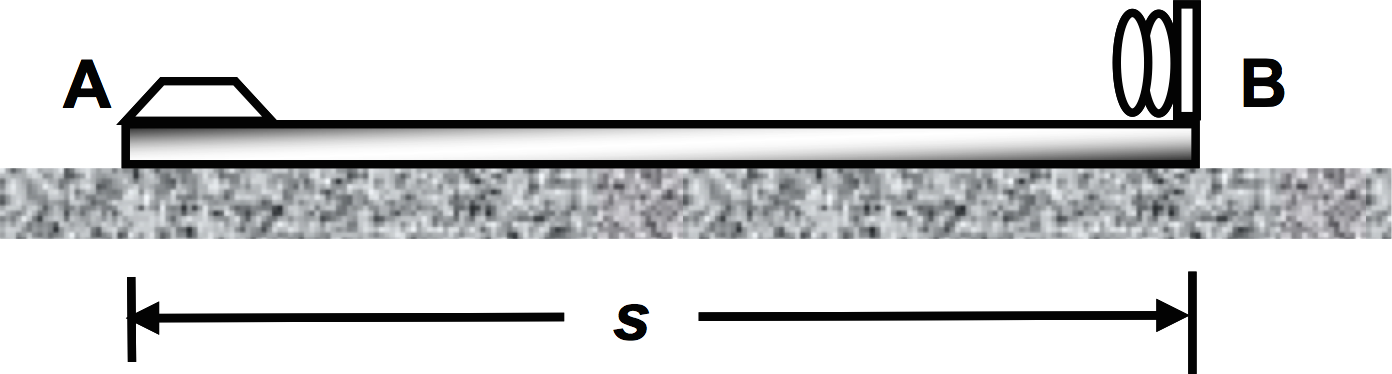
\includegraphics[width=\textwidth]{bumper.png}
\end{minipage}
\end{tabular}

\item
Object A is dropped from a height $h$. At the same instant object B is thrown vertically upward from the ground. Right before they collide in mid-air, the speed of A is three times the speed of B. Which of the following can be the height where the collision occurs?
\begin{enumerate}
\item $\displaystyle \frac{2h}{3}$
\item $\displaystyle \frac{h}{\sqrt{3}}$
\item $\displaystyle \frac{3h}{4}$
\item $\displaystyle \frac{h}{2}$
\item $\displaystyle \frac{h}{4}$
\end{enumerate}

% --- F=ma Question ---
% \item
% A uniform circular ring of radius $R$ and linear mass density $\lambda$ is fixed in place. A particle is placed on the axis of the ring at a distance much greater than $R$ and allowed to fall toward the ring under the influence of the ring's gravity. The particle achieves a maximum speed $v$. The ring is replaced with one of linear mass density $2\lambda$ and radius $2R$, and the experiment is repeated. What is the new maximum speed of the particle?
% \begin{enumerate}
% \item $v/2$
% \item $v/\sqrt{2}$
% \item $v$
% \item $\sqrt{2}v$
% \item $2v$
% \end{enumerate}

% -------------------------
\item
A force $F$ is used to hold two blocks of mass $m_1$ and $m_2$ on an incline as shown in the diagram. The plane makes an angle $\theta$ with the horizontal and $F$ is perpendicular to the plane. The coefficients of static friction between the plane and the block $m_2$ and between the two blocks are both equal to $\mu$ with $\mu < \tan\theta$. What is the minimum force $F$ necessary to keep both blocks at rest?

\begin{tabular}{l r}

\begin{minipage}{0.6\textwidth}
\begin{enumerate}
\item $\mu\left(m_1+m_2\right)$
\item $\left(m_1+m_2\right)g\cos\theta$
\item $\displaystyle m_1g\left(\frac{\sin\theta}{\mu}-\cos\theta\right)$
\item $\displaystyle m_2g\left(\frac{\sin\theta}{\mu}-\cos\theta\right)$
\item $\displaystyle \left(m_1+m_2\right)g\left(\frac{\sin\theta}{\mu}-\cos\theta\right)$
\end{enumerate}
\end{minipage} &
\begin{minipage}{0.3\textwidth}
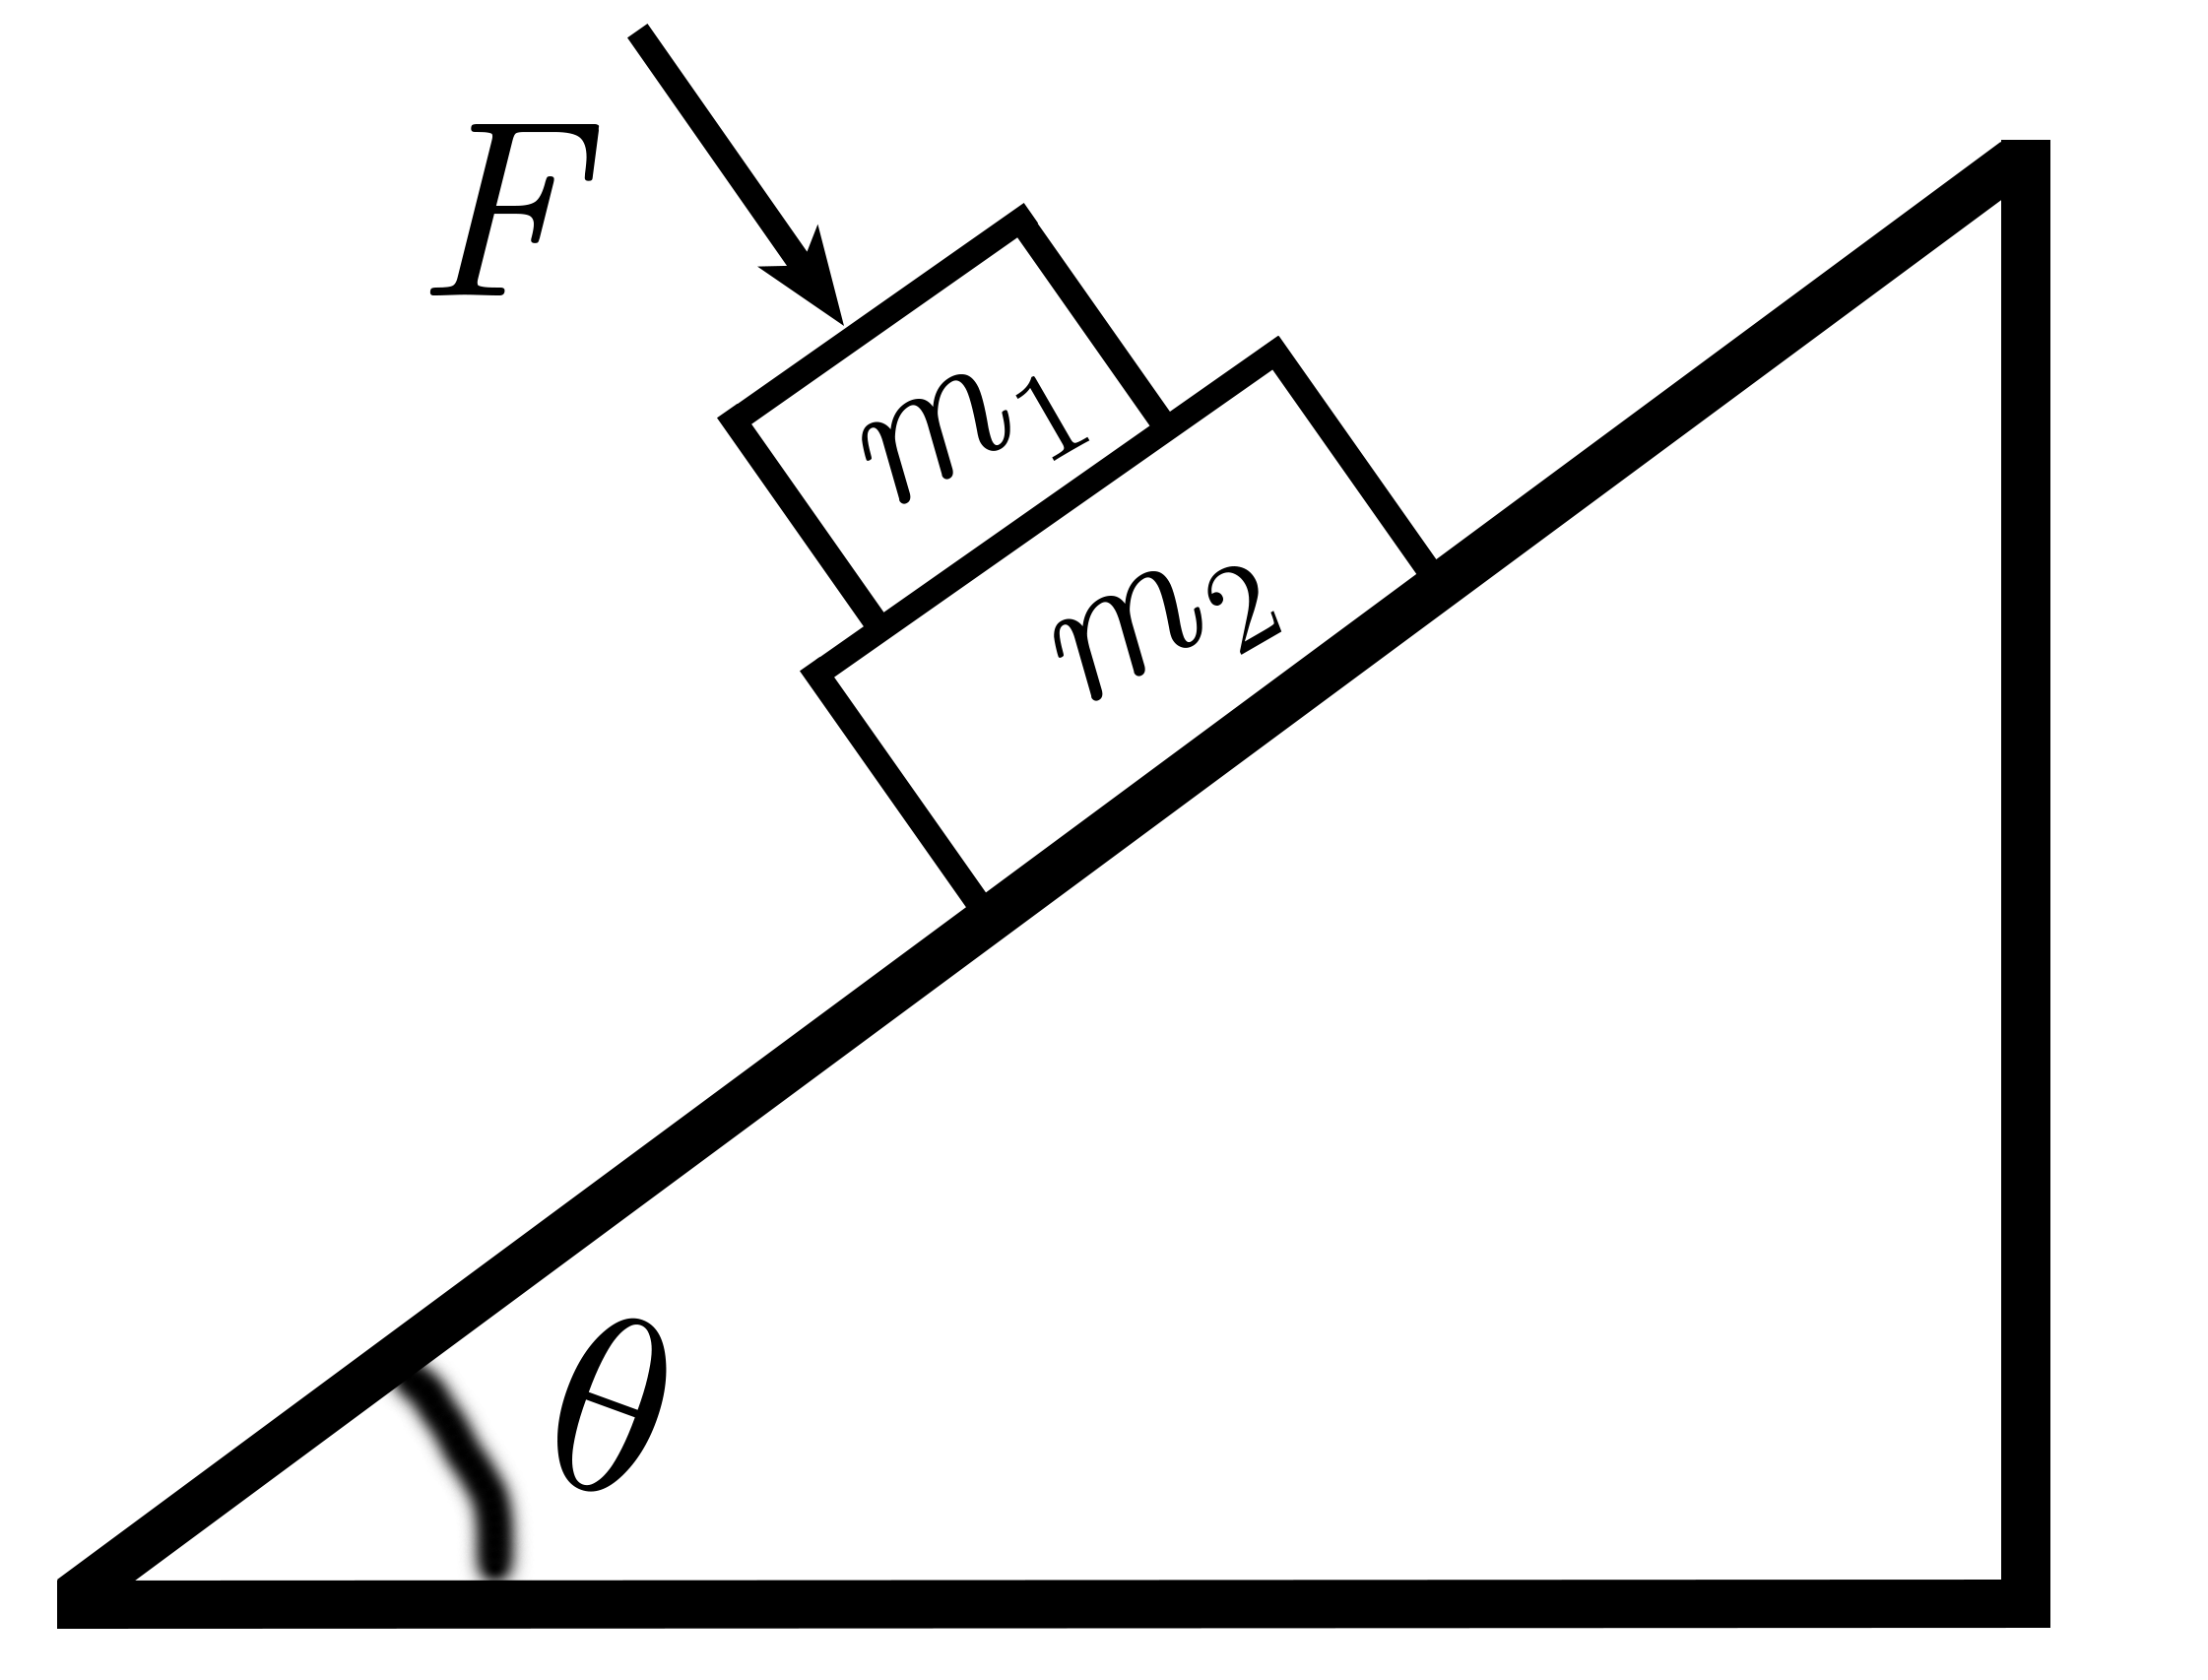
\includegraphics[width=\textwidth]{incline.png}
\end{minipage}
\end{tabular}

\item
As shown, a big box of mass $M$ is resting on a horizontal smooth floor. On the bottom of the box there is a small box also of mass $M$. The block is given an initial peed $v_0$ relative to the floor, and starts to bounce back and forth between the two walls of the box. Find the final speed of the box when the block has finally come to rest in the box.

\begin{tabular}{l r}

\begin{minipage}{0.5\textwidth}
\begin{enumerate}
\item 0
\item $v_0$
\item $v_0$/2
\item $v_0$/3
\item $v_0$/4
\end{enumerate}
\end{minipage} &
\begin{minipage}{0.4\textwidth}
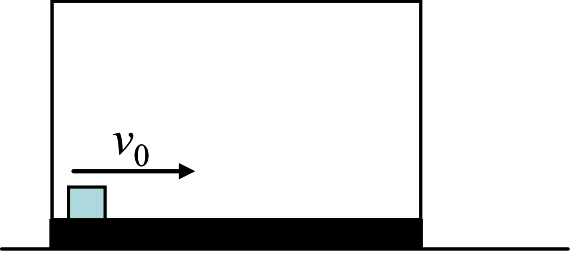
\includegraphics[width=\textwidth]{box-lg.png}
\end{minipage}
\end{tabular}

\item
Two astronauts, A and B, both with mass of 60 kg, are moving along a straight line in the same direction in a ``weightless'' spaceship. Relative to the spaceship the speed of A is 2 m/s and that of B is 1 m/s. A is carrying a bag of mass 8 kg with him. To avoid collision with B, A throws the bag with a speed $v$ relative to the spaceship toward B and B catches it. Find the minimum value of $v$.

\begin{tabular}{l r}

\begin{minipage}{0.5\textwidth}
\begin{enumerate}
\item 7.8 m/s
\item 26.0 m/s
\item 14.0 m/s
\item 9.2 m/s
\item 5.5 m/s
\end{enumerate}
\end{minipage} &
\begin{minipage}{0.4\textwidth}
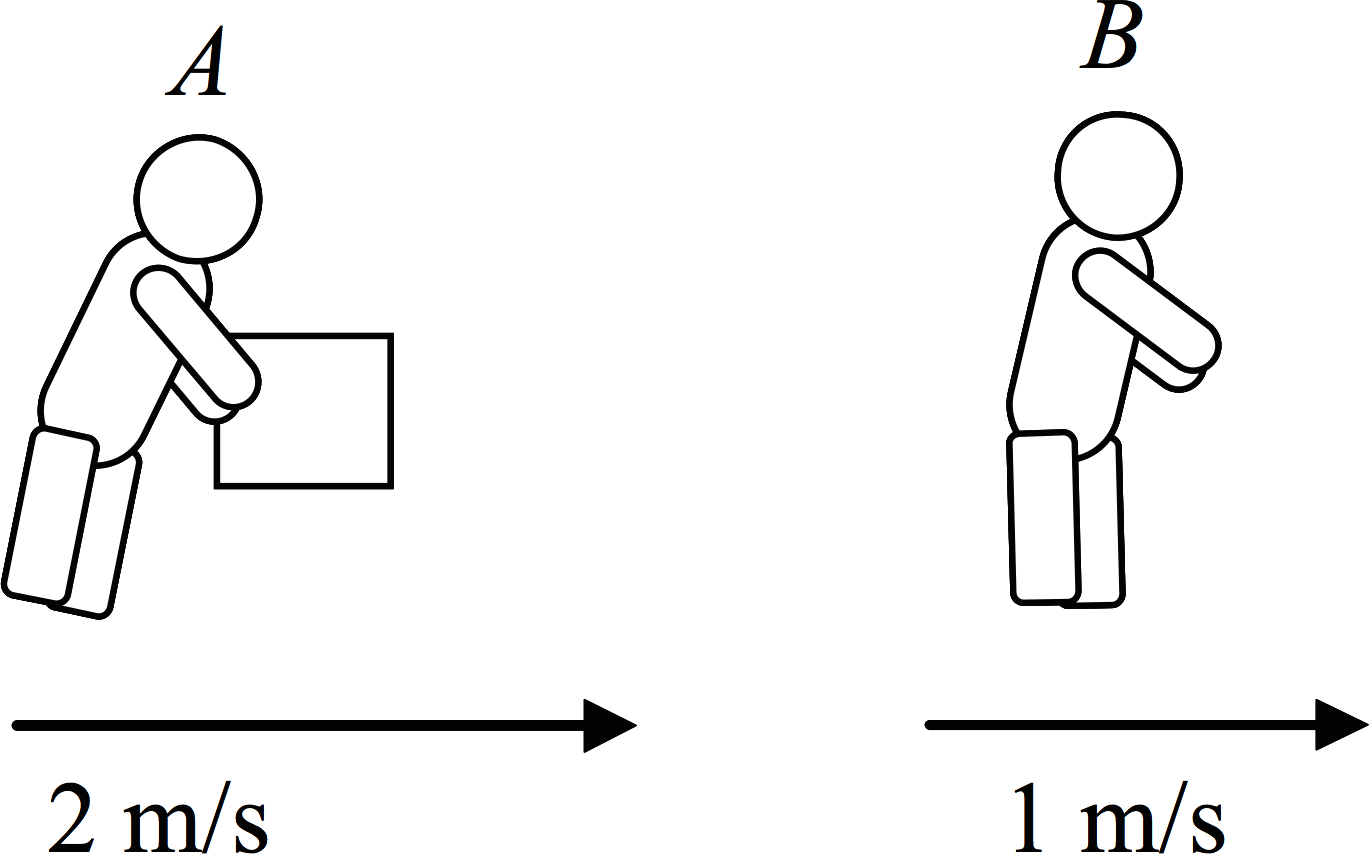
\includegraphics[width=\textwidth]{astronauts.png}
\end{minipage}
\end{tabular}

\vfill
\newpage

\item
As shown in the diagram, a man pushes forward on the compartment which is accelerating uniformly to the left relative to the ground. The man stays at rest relative to the compartment. Which of the following statements in respect to the ground reference frame is correct?

\begin{tabular}{l r}

\begin{minipage}{0.5\textwidth}
\begin{enumerate}
\item The man does positive work on the compartment.
\item The man does negative work on the compartment.
\item The man does zero work on the compartment.
\item It cannot be determined
\item Both (a) and (c) can be correct.
\end{enumerate}
\end{minipage} &
\begin{minipage}{0.4\textwidth}
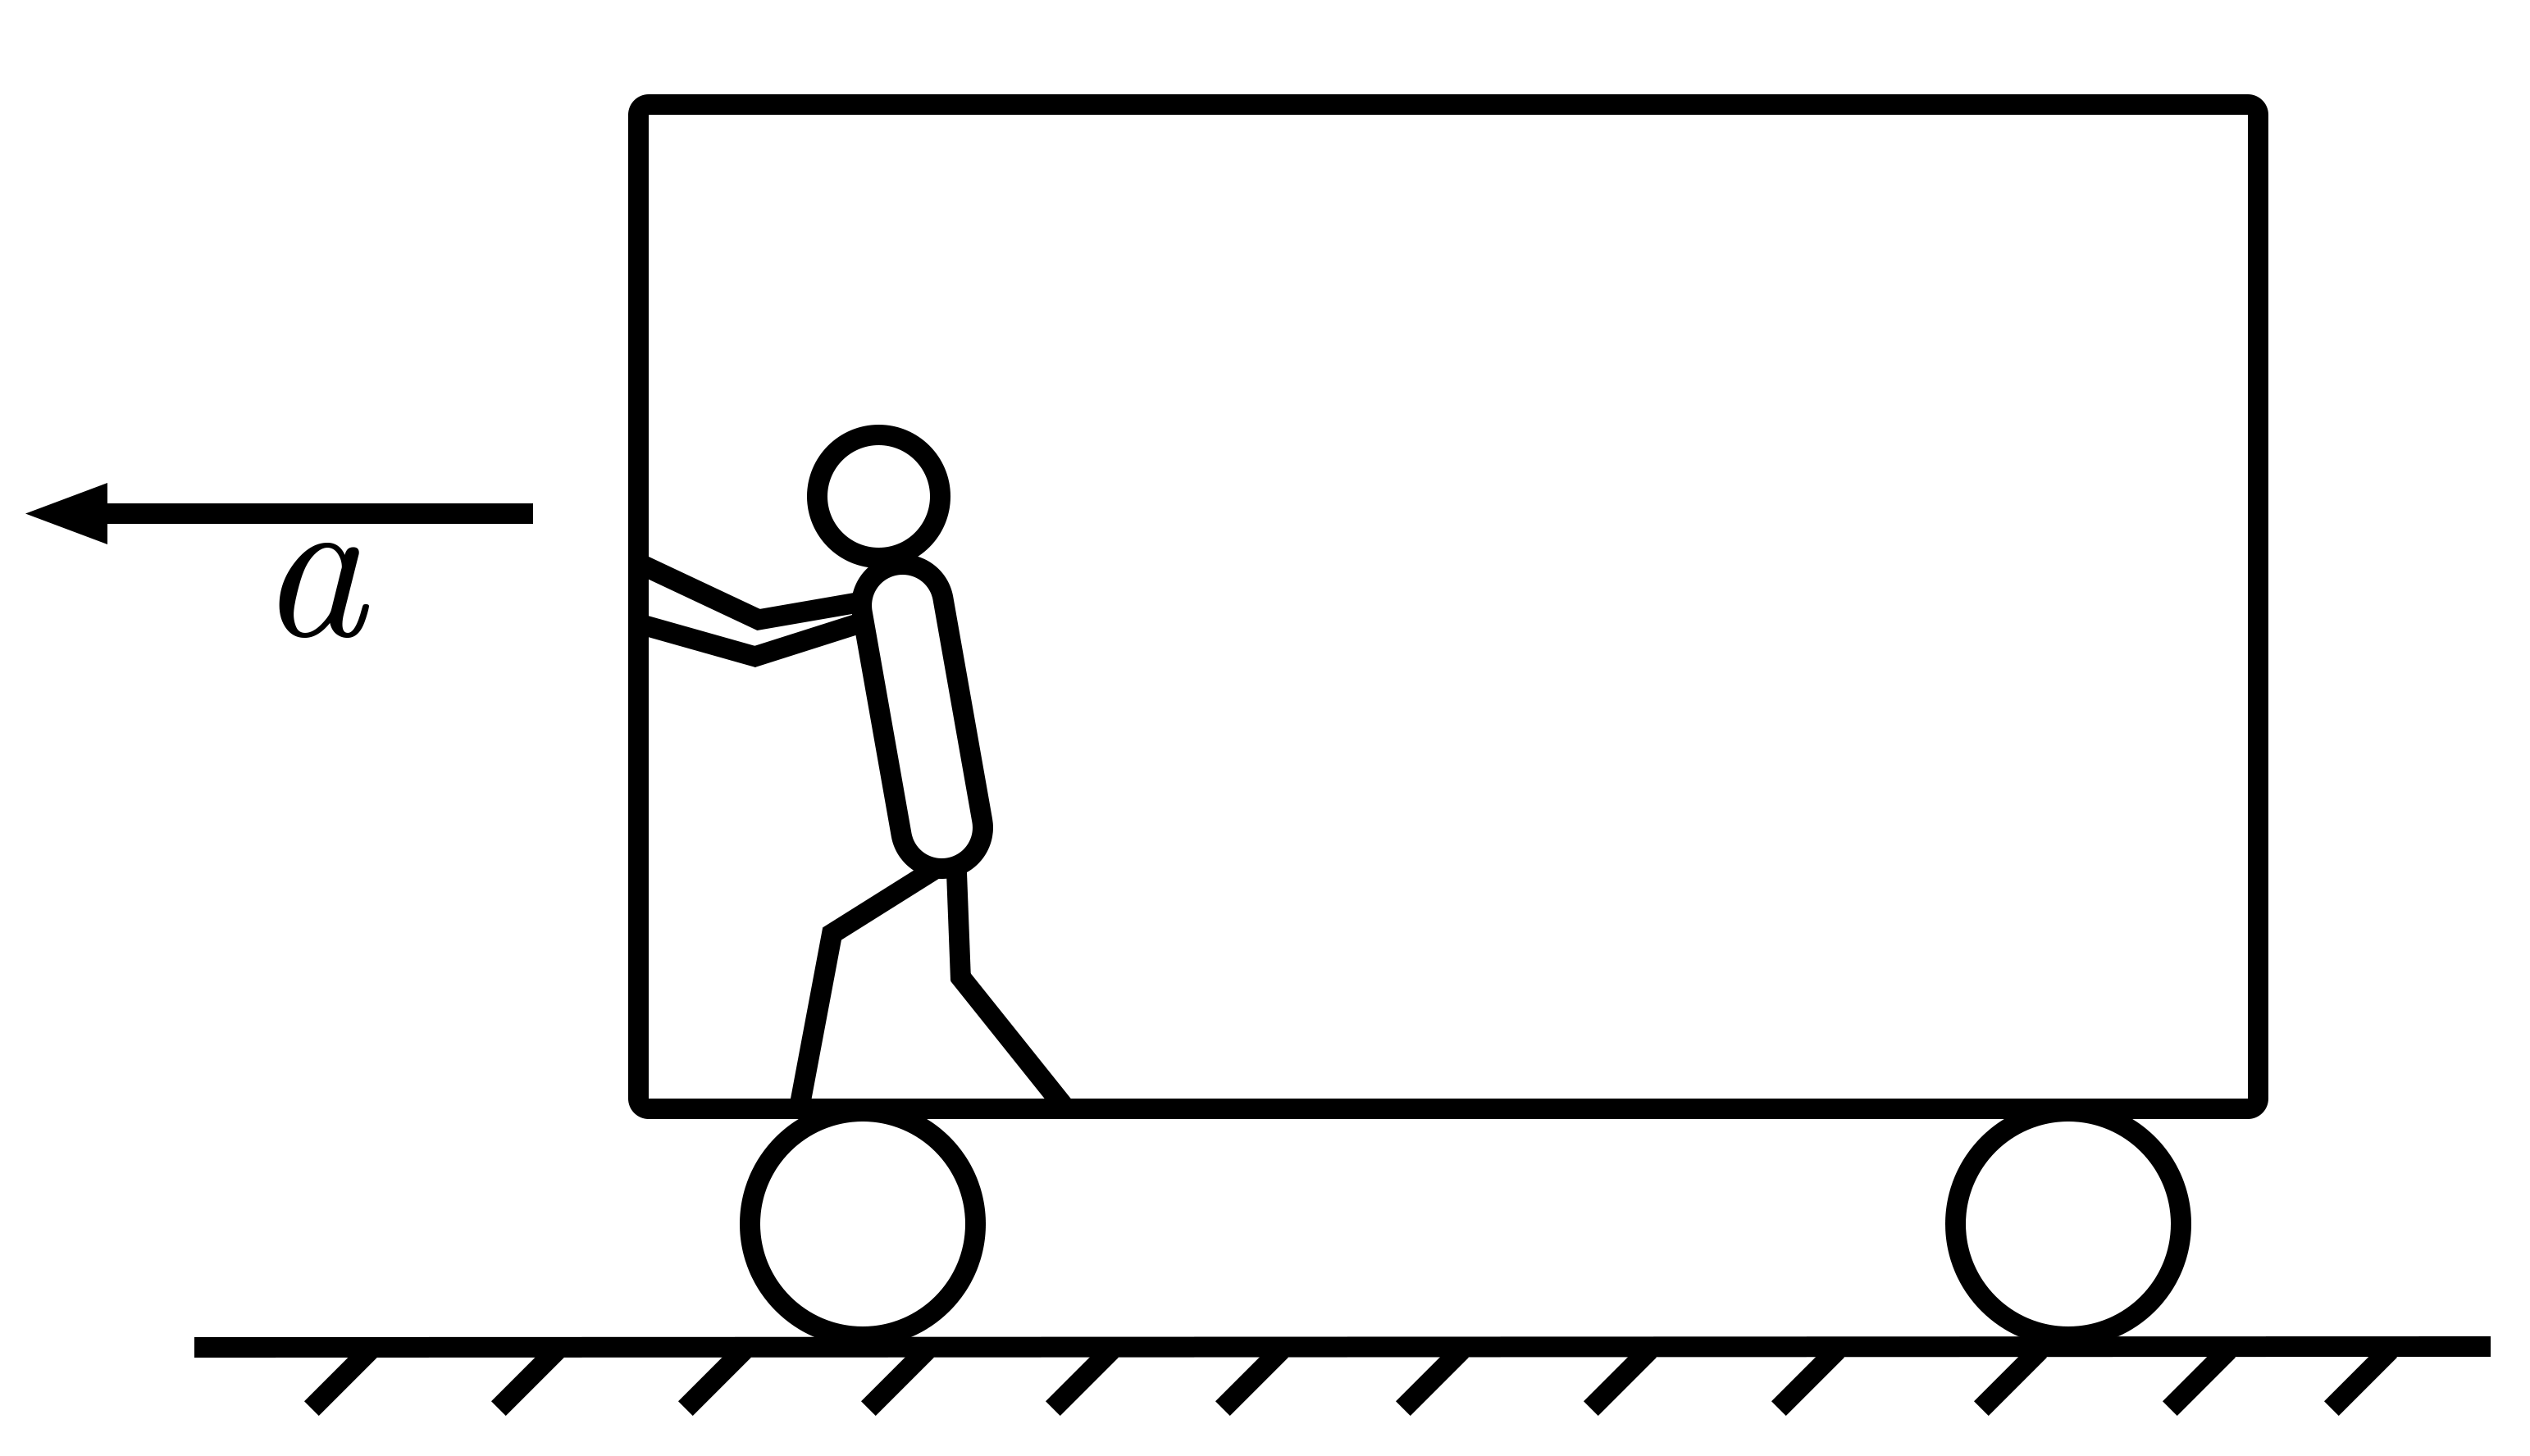
\includegraphics[width=\textwidth]{compartment.png}
\end{minipage}
\end{tabular}

\item
As shown in the figure, AB $= 3.5$ m, AC $=3.0$ m, AD $= 0.5$ m. The two rods AC and BC weight 200 N each. The floor is frictionless. Find the tension in the rope.

\begin{tabular}{l r}

\begin{minipage}{0.5\textwidth}
\begin{enumerate}
\item 280 N
\item 500 N
\item 150 N
\item 302 N
\item 180 N
\end{enumerate}
\end{minipage} &
\begin{minipage}{0.4\textwidth}
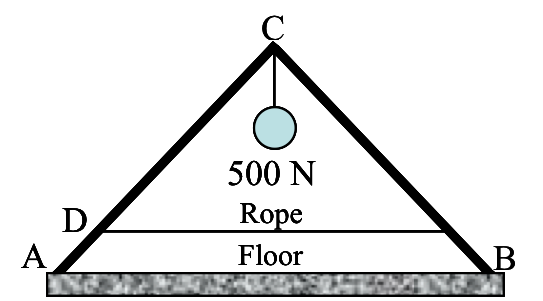
\includegraphics[width=\textwidth]{triangle.png}
\end{minipage}
\end{tabular}


\item
A small weight of mass $2M$ is attached to the bottom of a hollow sphere of mass $M$ and radius $R$. Half of the sphere is submerged when floating in water. Find the period $T$ of the simple harmonic oscillation of the sphere in the vertical direction.
\begin{enumerate}
\item $\displaystyle 2\pi\sqrt\frac{R}{2g}$
\item $\displaystyle 2\pi\sqrt\frac{3R}{2g}$
\item $\displaystyle 2\pi\sqrt\frac{R}{g}$
\item $\displaystyle 2\pi\sqrt\frac{2R}{3g}$
\item $\displaystyle 2\pi\sqrt\frac{R}{3g}$
\end{enumerate}
\end{enumerate}
\end{document}
